\chapter{The Baltic Sea}
\label{kap-einleitung}

In the previous chapters, an idealized process study with the help of a 
numerical model was carried out (section \ref{kap-slope}) and observations of 
the discussed process in an existing data set from the East China Sea were 
reproduced (section \ref{kap-jgr}). Besides model studies, several field work 
campaigns were performed in the context of this thesis. The measurements were 
carried out in coastal areas of the Western Baltic Sea. Prior to the discussion 
of the obtained data in the next chapter, an introduction on the evolution of 
the Baltic Sea and the present hydrological conditions is given in this 
chapter, and the sedimentology and prevailing hydrodynamic processes which are 
characteristic in parts of the Western Baltic Sea are highlighted.

\section{History and Present State}

The Baltic Sea emerged from a subglacial lake at the end of the Weichselian Ice 
Age, approximately 12,000 BP, and has since gone through several stages of 
salty and brackish sea states or fresh water conditions, depending on whether a 
connection to the open ocean was established or not. Indicators for this 
alternations are, amongst others, changes in the benthic communities, and so the 
nomenclature of the evolution stages was often determined by the prevailing 
species.

With the retreat of the glaciers at the end of the Weichselian Ice Age, a 
subglacial lake, together with water from the rapidly melting glaciers, formed 
the \textit{Baltic Ice Lake}. Land uplift, that followed the deglaciation, 
formed a landbridge between Sweden and the main land 11,200 BP, damming the 
Baltic Ice Lake. Sea level was raised by glacial melt water until the lake began 
to drain over the Öresund sill. Presumably, a lowering of the water level by 25 
to 28 m by drainage through a channel near Mt. Billingen in central Sweden 
happened very rapidly around 10,300 BP, when the retreating ice margin collapsed 
\citep[][]{bjoerk95,tikkanen2002} and a connection to the sea was opened. 

This new stage of the Baltic with a lower sea level is known as \textit{Yoldia 
Sea} (from the marine mollusc \textit{Portlandia (Yolida) arctica} 
\citep[][]{schoning2001}). There are no indicators for salt water entrainment 
into the Yoldia Sea until global sea level rise and deglaciation formed a 
connection through the Närke Strait 300 years later \citep[][]{schoning2001}. 
This lead to brackish water conditions followed by decreasing salinity after the 
straits had become too narrow to allow water exchange another 100 to 300 years 
later \citep[][]{bjoerk95}.

After the glaciers retreated, uplift of the land was not be compensated by 
global sea level rise. Connection to the ocean was closed again around 9,500 BP, 
and the regime shifted to fresh water conditions again, now called 
\textit{Ancylus Lake} (after the freshwater gastropod \textit{Ancylus 
fluviatilis} \citep[][]{tikkanen2002}). Although narrow outlets existed, the 
surface of the Ancylus Lake rose up to 10 m above global sea level, inundating 
extensive areas of land. This phase, called the Ancylus Transgression, ended 
around 9,200 BP, when the sea level height exceeded the height of the Darss Sill 
and water began to flow out through an evolving river system in the land 
connection between Sweden and Germany \citep[][]{tikkanen2002}. Around 9,000 BP 
this so-called Ancylus Regression ended when the water level reached global sea 
level. The connection to the ocean through the river system remained, but no 
extensive saline intrusion happened for the next 1,000 years.

Ongoing global sea level rise deepened the connection between the Baltic Basin 
and the open ocean, letting more and more saline water enter the Ancylus Lake. A 
short transition stage called \textit{Mastogloia Sea} (\textit{Mastogloia} are 
diatoms that live in slightly saline conditions \citep[][]{eronen2001}) was 
followed by the \textit{Litorina Sea} (named after the brackish water gastropod 
\textit{Littorina littorea} \citep[][]{eronen2001}), when a great extent of 
saline water entered the Baltic basin through the Straits of Denmark in 7,500 BP 
\citep[][]{bjoerk95}. Transgression took place until the rise in ocean levels 
ended 6,000 to 5,000 BP. When the Straits of Denmark became shallower, as land 
uplift continued, water exchange was reduced and salinity in the Litorina Sea 
declined down to the present brackish state in 4,000 BP, at first named 
\textit{Limnea Sea} (from the snail \textit{Lymnaea ovata}), and finally, since 
500 BP, \textit{Mya Sea} (after the Northern American clam \textit{Mya 
arenaria}, which was brought into the Baltic by Viking ships 
\citep[][]{bjoerck2008}).

\begin{figure}[ht]
 \flushleft
 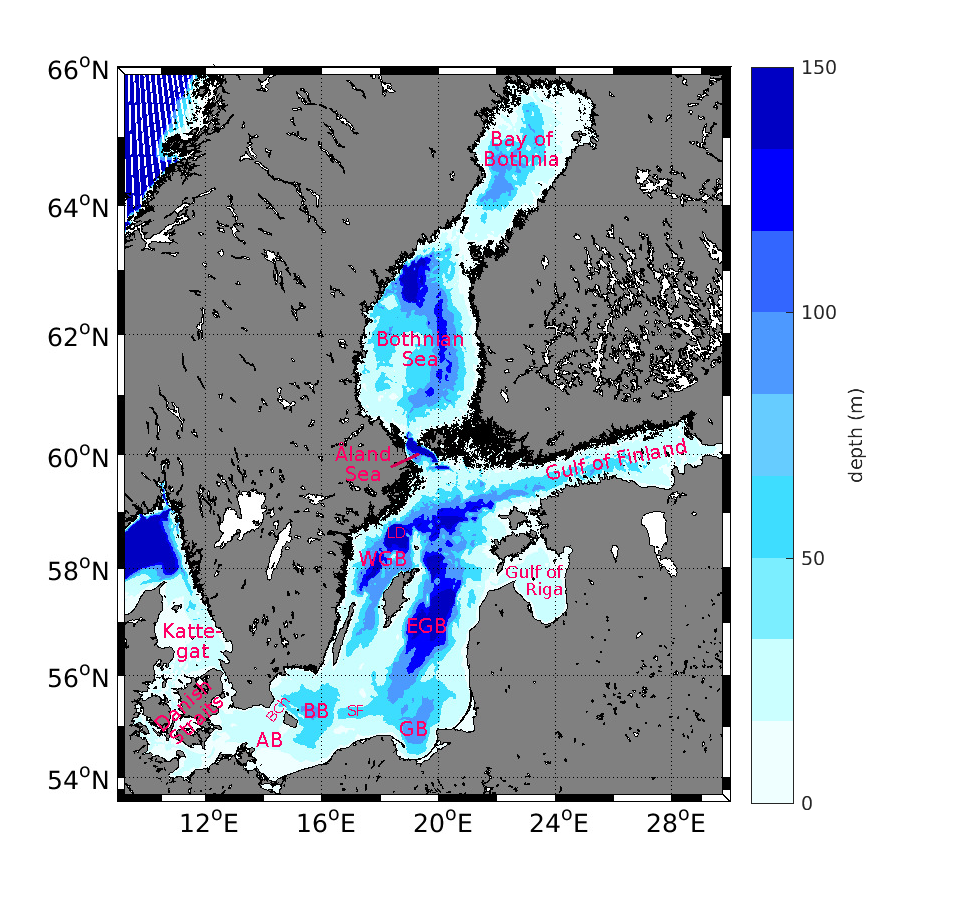
\includegraphics[width=17cm]{bilder/baltic.pdf}
 \caption{Topographic map of the Baltic Sea. Abbreviations stand for Arkona 
Basin (AB), Bornholm Channel (BCh), Bornholm Basin (BB), S\l upsk Furrow (SF), 
Gda\`{n}sk Basin (GB), Eastern Gotland Basin (EGB), Landsort Deep (LD) and 
Western Gotland Basin (WGB).}\label{balticmap}
\end{figure}

Today, the Baltic Sea has an extent of $4.2 \times 10^{5} \, \text{km}^2$ 
\citep[][]{balticsea} and is connected to the North Sea via the Danish Straits: 
the \O resund and the Great and Little Belt together with the Fehmarn Belt. The 
climate is humid: Annual precipitation adds around 224 $\text{km}^3$ of water to 
the Baltic Sea, evaporation amounts to only 184 $\text{km}^3$. River discharge a 
total of 436 $\text{km}^3$ water per year. \citep[][]{reissmann2009}. An 
exchange flow takes place, where brackish water leaves the Baltic near the 
surface (annually around 947 $\text{km}^3$) and saline North Sea water enters at 
the bottom (nearly 500 $\text{km}^3$ a year on average, but frequency and 
strength of inflow events differ dramatically over time, highly dependent on 
short term weather conditions). Two shallow sills, the Dr\o gden Sill (7 m deep, 
values in brackets refer to the local depth in the following) and the Darss Sill 
(18 m) form the passage to the first of several basins, the Arkona Basin (45 m), 
through which the North Sea water propagates as a deep gravity current 
(see \fig{balticmap}). Through 
the Bornholm Channel, the Arkona Basin is connected to the Bornholm Basin (80 
m), from where the bottom current flows over the S\l upsk Sill (60 m) and 
through the approximately 80 km long S\l upsk Furrow (90 m) southeast into the 
Gda\`{n}sk Basin (110 m) and northeast into the Eastern Gotland Basin (250 m). 
From there, the deep current can enter the easterly Gulf of Riga or the Western 
Gotland Basin, wherein the Landsort Deep (with 490 m the deepest point in the 
Baltic Sea) is located. The Gulf of Finnland forms the eastern boundary of the 
Baltic Sea and north of the Gotland Basin, the \r{A}land Sea separates the 
Baltic Proper in the south from the Bothnian Sea and the Bay of Bothnia in the 
north \citep[][]{reissmann2009}. Salt water entering at the Darss Sill needs 
approximately 2--6 months to exchange the bottom water in the Gotland Basin 
\citep[][]{balticsea}.

The bathymetry of the Baltic Basin together with climate conditions and the 
exclusive water exchange via the Danish Straits leads to several notable 
features in the hydrographic conditions: Dense bottom water from the North Sea 
creates a permanent strong halocline that separates bottom from surface water, 
preventing ventilation of the water masses in the deep basins. Oxygen that 
enters through exchange with the atmosphere is not mixed below the halocline, 
leaving entraining North Sea water the only oxygen source. Large parts of the 
Baltic Sea become anoxic after long periods without significant salt water 
inflows, with severe implications on geochemical processes and the ecosystem of 
both the lower water column and the sediment-water interface. 

Since the only source of saline water are inflows from the North Sea, a 
salinity gradient is present across the Baltic Sea: The bottom current is 
entrained with overlying brackish water along its pathway (for example, volume 
of the gravity current increases by 53 \% when passing through the Arkona Basin, 
\citep[see][]{reissmann2009}), and slow entrainment of salt into the overlying 
water mass forms a NE--SW surface salinity gradient. Surface salinity drops from 
around 18 psu in the Danish Straits to 8 psu in the Arkona Basin, down to 6--7 
psu in the Eastern Gotland Basin and even below 3 psu in the Bay of Bothnia and 
the Gulf of Finnland \citep[][]{balticsea}.

\section{Major Baltic Inflow December 2014}

Saline water can enter the Baltic Sea in two different ways. Baroclinic inflows 
are triggered by the horizontal salinity gradient between North and Baltic Sea 
and occur at calm wind conditions, mostly in summer \citep[][]{reissmann2009}. 
The main impact on the ventilation of the deep sea is, however, subject to the 
barotropic inflow events, called Major Baltic Inflows (MBIs). Those MBIs occur 
irregularly and are caused by special meteorological conditions: Firstly, high 
air pressure over the Baltic region and strong winds in westerly direction cause 
the mean sea level in the Baltic to drop by up to 50 cm, imposing a gradient in 
sea level elevation between Kattegat and Arkona Basin. Secondly, several weeks 
of wind in easterly direction with strong gales \citep[][]{balticsea, 
reissmann2009, mohrholz2015} push saline and oxygen rich water into the Baltic 
Sea.
These conditions occur primarily between October and February. Since records 
started in 1897, MBIs were on a rather regular base up to the 1970s. After this, 
long periods without inflow events decreased oxygen supply in the Baltic basins 
drastically. The last MBIs were in 1993 and 2003, but they interrupted the 
anoxic conditions in the deep water only for short periods of time 
\citep[][]{schinke1998, mohrholz2015}.

In November 2014, medium to strong easterly winds forced an outflow of Baltic 
sea water and consequently a drop in mean sea level of 57 cm. At the beginning 
of December, the wind changed to heavily westerly wind, pushing a strong 
barotropic inflow of saline water into the Baltic Sea. The main inflow period 
lasted until Christmas. During that time, an overall amount of 320 $\text{km}^3$ 
water was imported into the Baltic Sea, carrying approximately 4 Gt salt. The 
MBI in 2014 was the third largest inflow event recorded since 1880 and has the 
potential to ventilate the entire deep water of the Baltic. 

\section{German Coastal Seas and Sediment}

General sedimentology and grain size distribution of parts of the Western 
Baltic Sea have 
been mapped in detail in a collaboration between the German maritime and 
hydrographic agency (BSH) and the Leibniz Institute for Baltic Sea Research 
(\fig{westernbaltic}). Prevailing sediments in this area reach from 
fine sand to silt. Although sediment distribution is rather inhomogeneous, some 
features related to the bathymetry are clearly visible. In the very shallow 
regions with water depth less than 20 m, predominately sandy sediments are 
found, while in the deeper basins finer silt is present.
As fine grained material is easily eroded, it is not likely to remain in highly 
energetic, shallow regions and is therefore transported into the deeper basins, 
where 
it accumulates \citep[][]{basys1}. This process is best visible at the 
transition from the Oder Bight to the Arkona Basin. It was found that the 20 m 
isobath seperates erosional from depositinal areas, and the muddy sediments 
accumulate below a regional halocline here \citep[][]{basys2}.

\begin{figure}[ht]
 \flushleft
 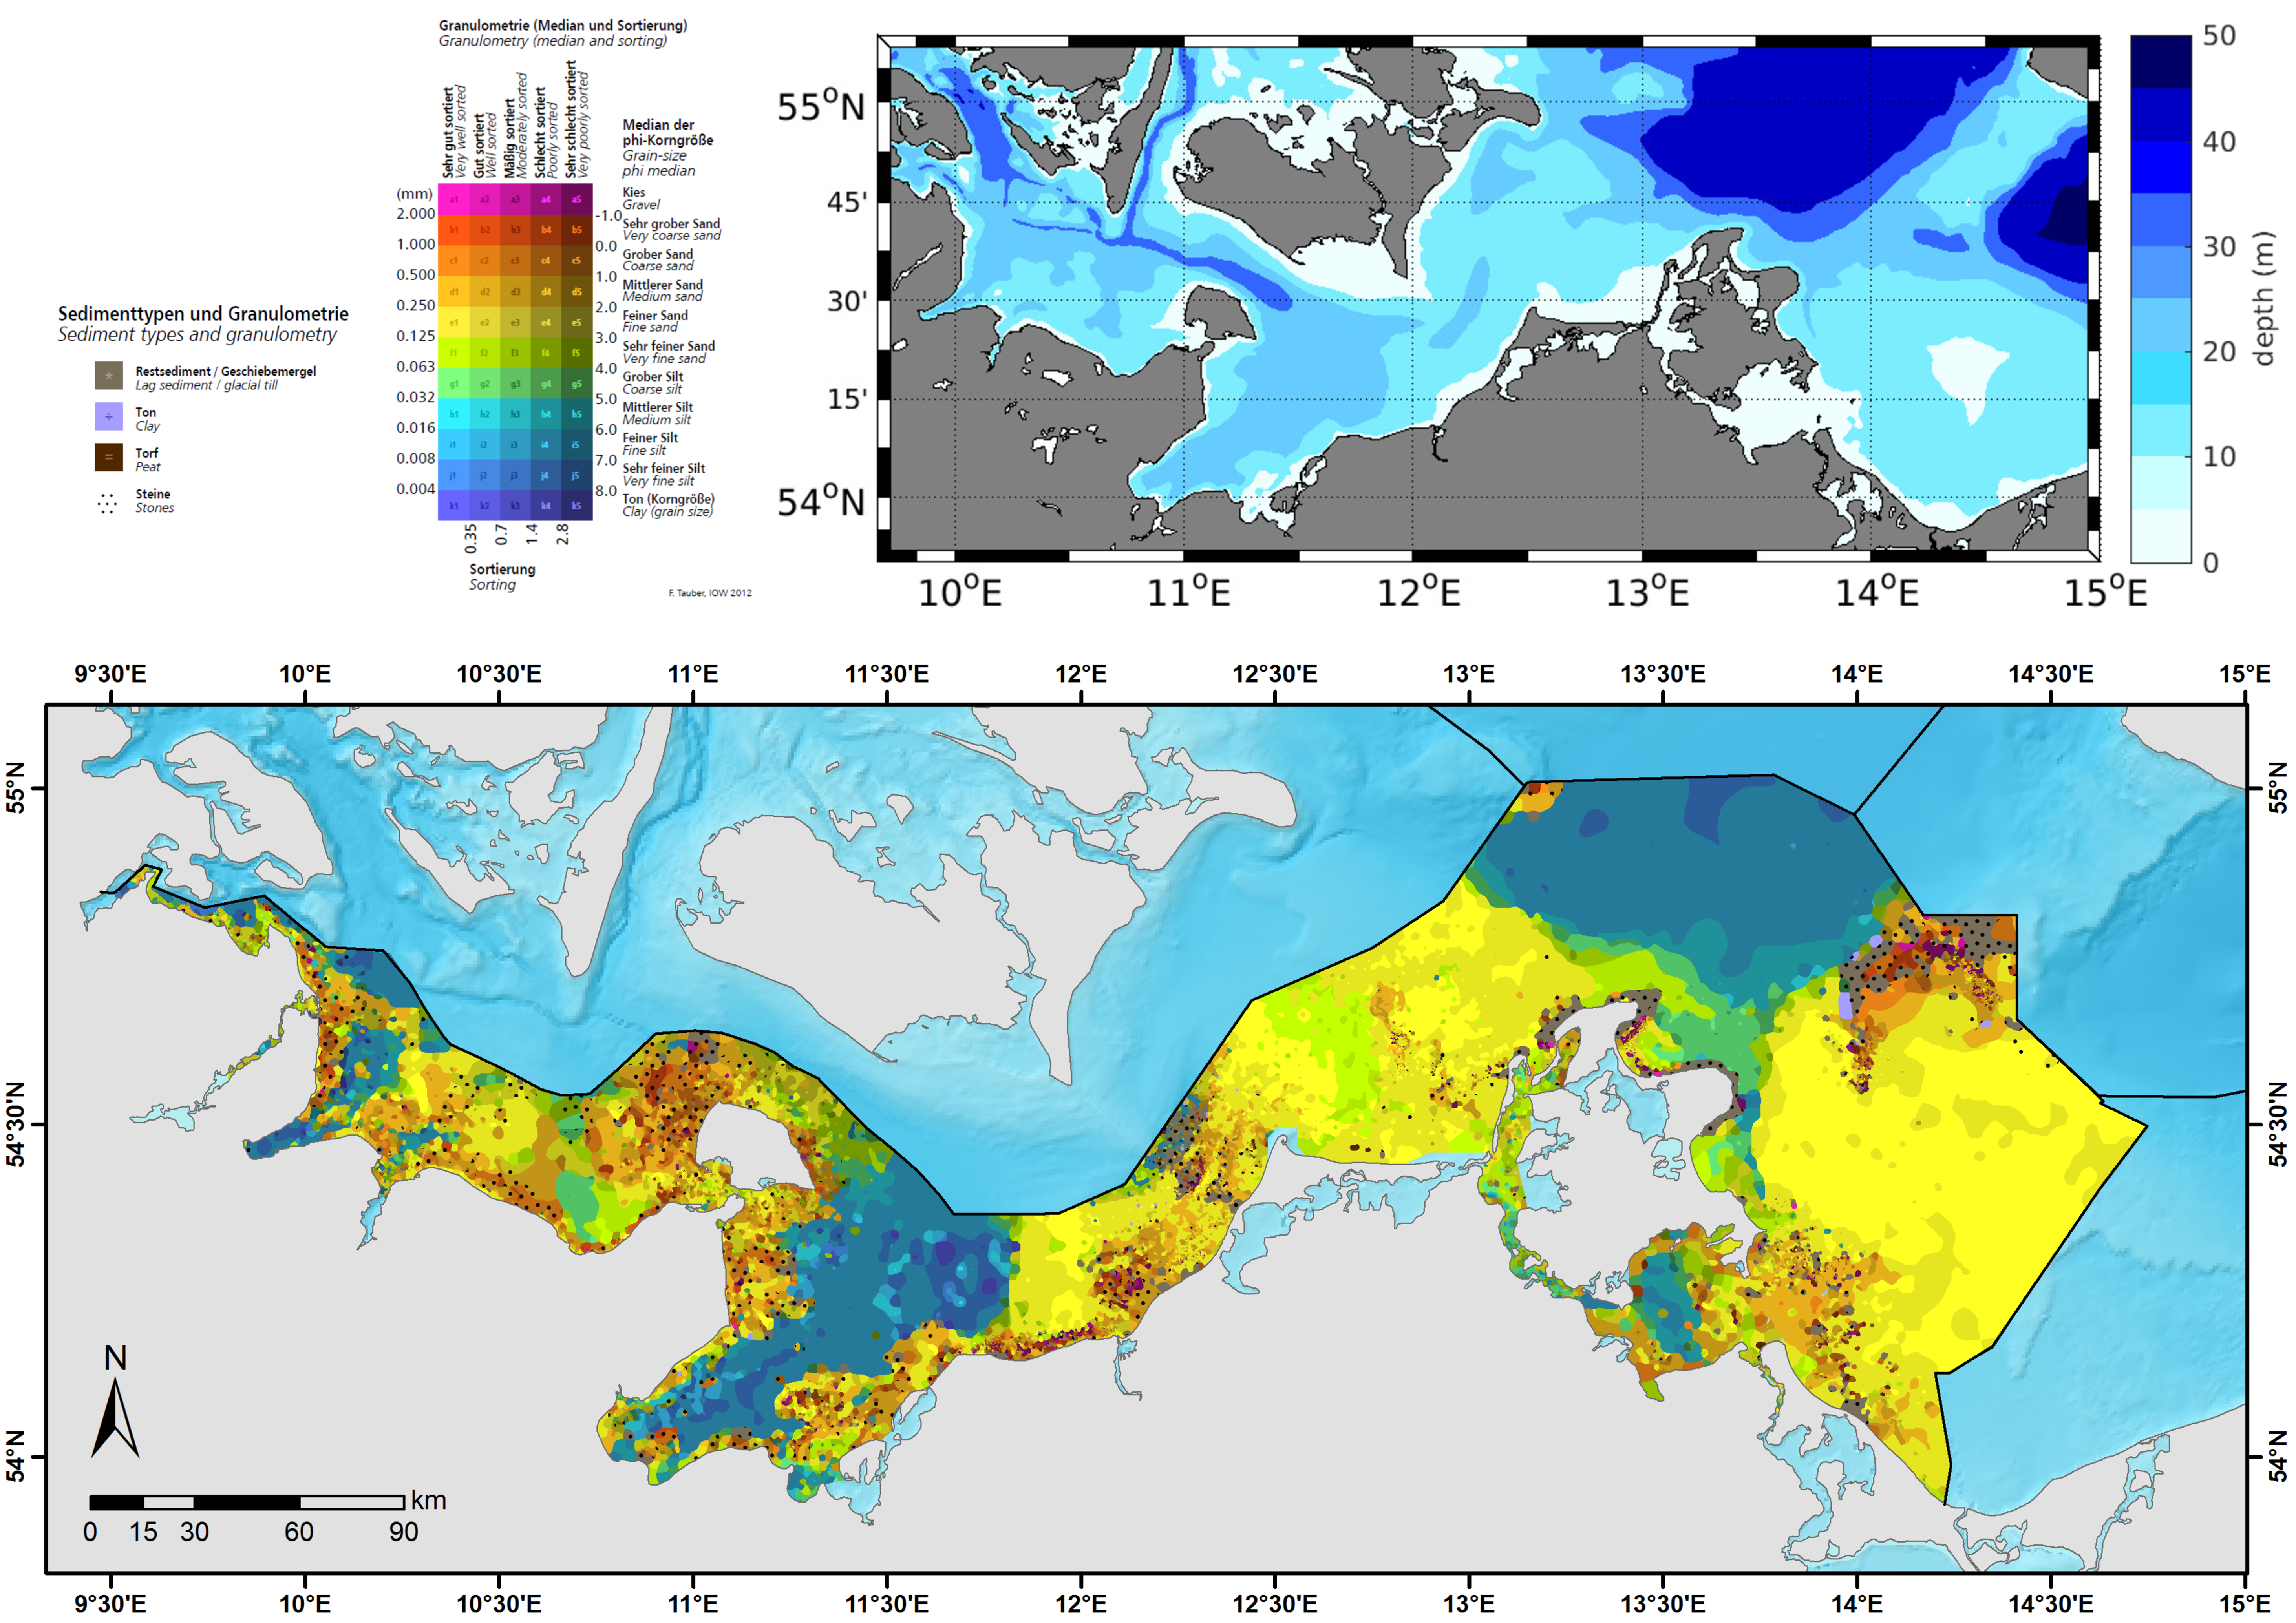
\includegraphics[width=15cm]{bilder/sediment.pdf}
 \caption{Topographic and sediment map of the Western Baltic 
Sea. Sediment data is taken from \citep[][]{tauber2012}}\label{westernbaltic}
\end{figure}